%%%%%%%%%%%%%%%%%%%%%%%%%%%%%%%%%%%%%%%%%%%%%%%%%%%%%%%%%%%%%%%%%%%%%%%%%%%%%%%%%%%%%%%%%
% Section 10: Installing New Devices
%	This section provides a detailed walkthrough on how to install new devices
%	to be used in RapidSmith2.
%%%%%%%%%%%%%%%%%%%%%%%%%%%%%%%%%%%%%%%%%%%%%%%%%%%%%%%%%%%%%%%%%%%%%%%%%%%%%%%%%%%%%%%%%
\newpage
\section{Installing New Device Files} \label{sec:installingNewDevices}
\graphicspath{{./techReportFigures/sec10_deviceInstallation/}}

The device files included with the RapidSmith2 installation (listed in
\autoref{sec:supportedDevices}) have been well-tested, and are great starting
points for new users. If you are new to RapidSmith2, it is \textit{strongly
encouraged} to start with these existing device files. However, RapidSmith2
also supports installing new devices for parts not listed in
\autoref{sec:supportedDevices}. To create a new RapidSmith2 device
file, four \texttt{Tincr} intermediate files are required:

\begin{enumerate}
  \item XDLRC
  \item Family Info XML
  \item Device Info XML
  \item Cell Library XML
\end{enumerate}

\noindent The contents and format of these files are described in
great detail in \autoref{sec:appendixXDLRC}, \autoref{sec:familyInfo},
\autoref{sec:deviceInfo}, and section \ref{sec:cellLibraryinDesignSection}
respectively, and will not be described here. For those that are curious about
what each file represents, refer to the listed appedices. The remainder of this
section documents the required steps to transform the \texttt{Tincr}
intermediate files into compact device files that can be loaded into
RapidSmith2.

\subsection{Creating New Device Files for Supported Families}
\label{sec:creatingNewSupportedDevices} 
Section \ref{sec:supportedDevices} gives a list of currently supported
families in RapidSmith2. If the device to install is \textbf{not} within a
supported family, see \autoref{sec:newFamilies} for how to add support for a
new family in RapidSmith2. Otherwise, a new device file can be added in five
easy steps:

\begin {enumerate}
\item Open Vivado in Tcl mode, and execute the \texttt{Tincr} command
\texttt{[::tincr::write\_xdlrc]}. An example usage is shown in
\autoref{lst:apdxAwriteXdlrc} for the Artix7 part \textit{xc7a100tcsg324-3}. The
``-max\_processes'' option is used to parallelize the operation so that it will
execute faster. This Tcl command can take a very long time to run (more than 24
hours for very large devices), and so running the command on a remote machine is
good practice. Be aware that these XDLRC files are massive, and 100 GB for the
largest XDLRC files is not uncommon. Make sure there is enough space on the
hard drive before generating the XDLRC for a device.

\end {enumerate}

\begin{lstlisting}[numbers=none, caption=XDLRC Generation Example, label=lst:apdxAwriteXdlrc] 
::tincr::write_xdlrc -part xc7a100tcsg324-3 -max_processes 4 -primitive_defs xc7a100tcsg324_full.xdlrc
\end{lstlisting}

\begin{enumerate}
\setcounter{enumi}{1} 
\item Run the \texttt{Tincr} command \texttt{[tincr::create\_xml\_device\_info]}
 to create a \textit{deviceInfo.xml} file for the part. Copy the generated
 \textit{deviceInfo.xml} file to the directory
 \textit{rapidSmithPath/devices/family}, where ``rapidSmithPath'' is the path to
 your RapidSmith2 installation and ``family'' is the corresponding Vivado
 family name (i.e. artix7, kintex7, virtex7, zynq, kintexu, virtexu,
 kintexuplus, virtexuplus, etc.)..

\item Run the device installer in RapidSmith2 and pass the newly created XDLRC
as an argument. An example command line usage is shown in
\autoref{lst:apdxAInstaller}. The device installer creates compact device files
that represent a Xilinx device from the XDLRC and \textit{deviceInfo.xml}
generated in the previous steps. Notice the two JVM command line arguments used
in the command. The first option (``-ea'') enables assertions for the code. It
is important to include this flag so that device file errors can be caught
during parsing. The second option (``-Xmx4096m'') sets how much memory the JVM
can use while running the installer. Since XDLRC files are quite large, the
memory usage of the installer grows very quickly. If the device installer fails
with an out of memory exception, you will need to increase the memory and
re-run the installer (up to 32 GB of memory may be required).
\end{enumerate}

\begin{lstlisting}[numbers=none, caption=RapidSmith2 device installer example
usage, label=lst:apdxAInstaller] 
java -ea -Xmx4096m edu.byu.ece.rapidSmith.util.Installer --generate file xc7a100tcsg324_full.xdlrc
\end{lstlisting}

\begin{enumerate}
\setcounter{enumi}{3}
\item Run the family builder in RapidSmith2 and pass the name of the newly
created part as a command line argument. An example usage is shown in
\autoref{lst:apdxAFamilyBuilder} for an Artix7 device. An \texttt{Artix7.java}
file (or whatever family your device is in) will already exist, but will be
updated with new sites and tile types from the newly installed part.

\item The final step is to create a \textit{cellLibrary.xml} file, which details
all Xilinx primitives that can target the device. \autoref{sec:cellLibraryGeneration}
demonstrates how to generate a new cell library. Copy the generated cell library
to the corresponding family folder of the device and rename it to
``cellLibrary.xml.''

\end{enumerate}

\begin{lstlisting}[numbers=none, caption=Family builder example usage,
label=lst:apdxAFamilyBuilder] 
java edu.byu.ece.rapidSmith.util.FamilyBuilders xc7a100tcsg324
\end{lstlisting}

\vspace{.3cm}

\noindent Once the device installer is done executing, the compact devices files
are stored in the corresponding family directory of the RapidSmith2 ``devices''
folder. For example, the device files generated from the example part
\textit{xc7a100tcsg324-3} are stored in the ``artix7'' sub-directory.
\autoref{lst:apdxADeviceFiles} shows the two device files that are created
after the device installer is run. The file ending in ``\_db.dat'' contains the
serialized \texttt{Device} data structures for RapidSmith2. The file ending in
``\_info.dat'' contains additional serialized data (such as reverse wire
connections) that can be optionally loaded with the device.

\begin{lstlisting}[numbers=none, caption=Generated RapidSmith2 device files,
label=lst:apdxADeviceFiles] 
[ttown523@CB461-EE09968:artix7] ls
cellLibrary.xml familyInfo.xml |\textbf{xc7a100tcsg324\_db.dat}| |\textbf{xc7a100tcsg324\_info.dat}|
\end{lstlisting} 

\subsection{Supporting New Device Families} \label{sec:newFamilies}
Vivado 2016.2 supports implementing FPGA designs on devices for the following
families (also called architectures):

\begin{multicols}{2}
	\begin {itemize}
	  \item \textbf{Artix7 (artix7)}
	  \item \textbf{Kintex7 (kintex7)}
	  \item \textbf{Virtex7 (virtex7)}
	  \item \textbf{Zynq (zynq)}
	  \item \textbf{Kintex Ultrascale (kintexu)}
	  \item \textbf{Virtex Ultrascale (virtexu)}
	  \item Kintex Ultrascale+ (kintexuplus)
	  \item Virtex Ultrascale+ (virtexuplus)
	\end{itemize}
\end{multicols}

\noindent The name in parentheses is the Vivado Tcl name for the family. Bolded
items are families that are currently supported in RapidSmith2 and
\texttt{Tincr}. To add RapidSmith2 support for another Vivado family, follow the
steps listed below. \textbf{NOTE: In general, you should not be adding support
for a new family as a general user of RapidSmith2. Instead, create an issue at the
RapidSmith2 GitHub repository and the maintainers of RapidSmith2 in the BYU CCL
lab will add support. The following instructions are intended for BYU students
only}.

\begin {enumerate}
  \item Create the primitive definitions of the family using VSRT. The VSRT user
  guide is given in located at {\color{blue}\url{
  https://github.com/byuccl/RapidSmith2/tree/master/doc}}.
  
  \item Copy the primitive definitions created in step (1) to the
   directory \textit{tincrPath/cache/family/primitive\_defs}, where
   ``tincrPath'' is the path to your \texttt{Tincr} installation and ``family''
   is the Vivado Tcl name for the family of the primitive defs just generated
   (shown in parentheses above).
   
   \item Create the \textit{familyInfo.xml}. To do this, open Vivado in Tcl mode
   and run the command \texttt{[::tin\-cr::create\-\_xml\_family\_info]}. An
   example usage of the command is shown in \autoref{lst:apdxAFamilyInfo} for
   Kintex UltraScale. As the listing shows, there are three arguments to the
   command:
   
	\begin{itemize}
	  \item \textbf{familyInfo.xml}: The file name to store the generated family
	  info. The file ending ``.xml" will be appended if it is not included.
	  \item \textbf{kintexu}: The Vivado family name.
	  \item \textbf{addedBels.txt} (Optional): The ``addedBels.txt" file that was
	  created during step (1). This file contains a list of added VCC/GND BELs for
	  each family.
	\end{itemize}    
\end{enumerate}

\begin{lstlisting}[numbers=none, caption=Family info example usage, label=lst:apdxAFamilyInfo] 
::tincr::create_xml_family_info familyInfo.xml kintexu addedBels.txt 
\end{lstlisting}


\begin{enumerate}
\setcounter{enumi}{3}    
    \item Modify the generated family info with a few hand edits. The required hand
    edits are broken down between Series7 and UltraScale devices in
    \autoref{sec:series7HandEdits} and \autoref{sec:ultrascaleHandEdits}
    respectively.

	\item Copy the generated \textit{familyInfo.xml} file to the directory
	\textit{rapidSmithPath/devices/family}, where ``rapidSmithPath'' is the path to
	your RapidSmith2 installation and ``family'' is the corresponding Vivado family
	name. Make sure the family info is named ``familyInfo.xml''. For example, if I
	generated a family info for the artix7 part ``xc7a100tcsg324'', I would copy
	the family info into the \textit{devices/artix7} directory.

	\item Follow the steps laid out in \autoref{sec:creatingNewSupportedDevices} to
	generate RapidSmith2 device files.
	    
	\item Run the Family Builder in RapidSmith2 (an example usage is shown in
	\autoref{lst:apdxAFamilyBuilder}). The Family Builder accepts one command line
	argument: a part name of a device in the family. Using the device files for
	the specified part, a Java file is created that contains all tile types and
	site types within the part. For example, the command in
	\autoref{lst:apdxAFamilyBuilder} will generate an \texttt{Artix7.java} file
	which can be used to find site and tile types as shown in
	\autoref{lst:apdxATypes}. Every family Java class includes a classifications
	section with the header ``/* ------ CLASSIFICATIONS GO HERE ------ */''. Below
	the header, tile and site classifications can be manually added to group
	similar site types together. The classifications for Artix7 are shown in
	\autoref{lst:apdxAClassifications} for reference.
	
\end{enumerate}

\begin{lstlisting}[language=java,numbers=none, caption=How to access SiteTypes
and TileTypes in RapidSmith2, label=lst:apdxATypes] 
SiteType siteType = Artix7.SiteTypes.SLICEL; 
TileType tileType = Artix7.TileTypes.CLBLL_L;
\end{lstlisting}

\begin{lstlisting}[language=java,numbers=none, caption=Device classifications
example, label=lst:apdxAClassifications] 
/* ------ CLASSIFICATIONS GO HERE ------ */ 
       // Tile Types
        _CLB_TILES.add(TileTypes.CLBLL_L);
        _CLB_TILES.add(TileTypes.CLBLL_R);
        _CLB_TILES.add(TileTypes.CLBLM_L);
        _CLB_TILES.add(TileTypes.CLBLM_R);

        _SWITCHBOX_TILES.add(TileTypes.INT_L);
        _SWITCHBOX_TILES.add(TileTypes.INT_R);

        _BRAM_TILES.add(TileTypes.BRAM_L);
        _BRAM_TILES.add(TileTypes.BRAM_R);
	
        _DSP_TILES.add(TileTypes.DSP_L);
        _DSP_TILES.add(TileTypes.DSP_R);
	
        _IO_TILES.add(TileTypes.LIOB33_SING);
        _IO_TILES.add(TileTypes.LIOB33);
        _IO_TILES.add(TileTypes.RIOB33);
        _IO_TILES.add(TileTypes.RIOB33_SING);

       // Site Types
        _SLICE_SITES.add(SiteTypes.SLICEL);
        _SLICE_SITES.add(SiteTypes.SLICEM);

        _BRAM_SITES.add(SiteTypes.RAMB18E1);
        _BRAM_SITES.add(SiteTypes.RAMB36E1);
        _BRAM_SITES.add(SiteTypes.RAMBFIFO36E1);

        _FIFO_SITES.add(SiteTypes.FIFO18E1);
        _FIFO_SITES.add(SiteTypes.FIFO36E1);
        _FIFO_SITES.add(SiteTypes.IN_FIFO);
        _FIFO_SITES.add(SiteTypes.OUT_FIFO);
        _FIFO_SITES.add(SiteTypes.RAMBFIFO36E1);
        
        _DSP_SITES.add(SiteTypes.DSP48E1);

        _IO_SITES.add(SiteTypes.IOB33);
        _IO_SITES.add(SiteTypes.IOB33S);
        _IO_SITES.add(SiteTypes.IOB33M);
        _IO_SITES.add(SiteTypes.IPAD);
        _IO_SITES.add(SiteTypes.OPAD);
\end{lstlisting}

\vspace{.3cm}
\noindent Once these steps are complete, RapidSmith2 will have full support for
the generated family. This means that device files for any part within the
family can be created.


\subsection{Series7 Family Info Hand Edits} \label{sec:series7HandEdits}
Due to complications with Vivado's Tcl interface,  several hand edits are
required to complete Series7 family info files. RapidSmith2 already
provides support for all Series7 families, but the required manual edits are
documented here in case they need to be regenerated in the future. 
    
\begin{enumerate}
  \item The first hand edit is to remove invalid alternate types. The only way
  to determine invalid alternate types in Vivado is to go site-by-site in the
  family info, select an instance of the site type in Vivado's device browser, and
  click the site type dropdown box (as shown in \autoref{fig:alternateTypes}).
  If there are any site types reported in the family info XML that are not
  shown in the GUI, they need to be removed from the XML. The Tcl commands
  shown in \autoref{lst:apdxASiteSelect} can be used to select a specific site
  type in Vivado to view its alternate types.

\end{enumerate}
 
\begin{lstlisting}[numbers=none, caption=Tcl commands to select a Vivado Site
object, label=lst:apdxASiteSelect]
Vivado% set site [lindex [get_sites -filter {SITE_TYPE==IPAD}] 0]
Vivado% select $site
\end{lstlisting}

\begin{figure}[b!]
  \centering
  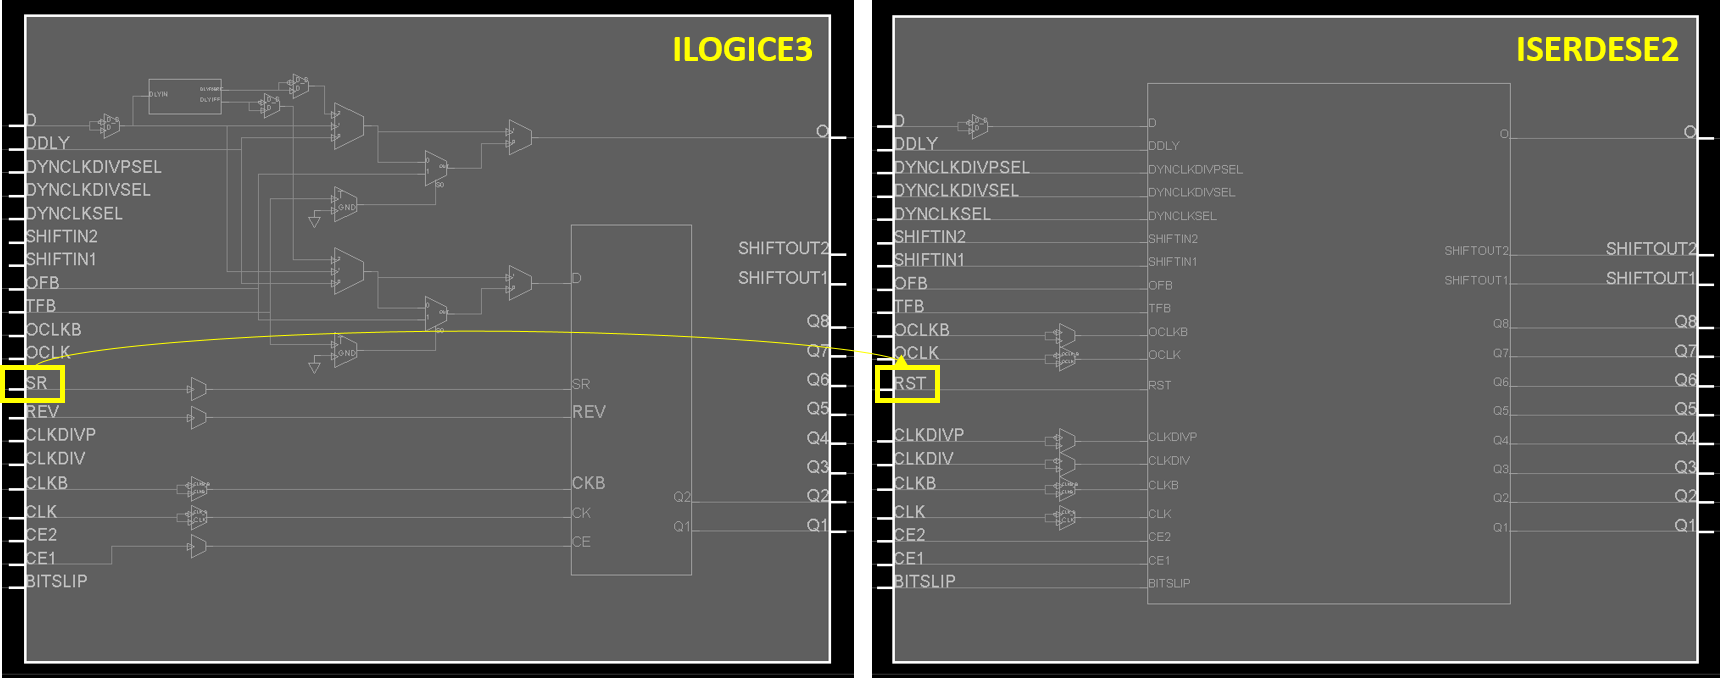
\includegraphics[width=\columnwidth]{alternatePinmap.png}
  \caption{Example Alternate Site Pin Renaming}
  \label{fig:alternatePinmap}
\end{figure}

\begin{enumerate}
\setcounter{enumi}{1}         
      \item  The second hand edit is to add alternate type pin mappings. When a
      site is changed to one of its alternate types in Vivado, the site pins can
      be renamed. An example is shown in \autoref{fig:alternatePinmap} for an
      IDELAYE3 site that has been changed to the alternate type ISERDESE2.
      Notice how the ``SR'' site pin has been renamed to ``RST'' in the figure.
      Unfortunately these pin renamings cannot be automatically extracted from
      Vivado's Tcl interface, and so must be added manually.
      \autoref{lst:apdxAPinmaps} shows how to add pin renamings to the family
      info XML using the ``pinmaps'' tag. To determine the actual pin
      mappings, the first step is to open two instances of the Vivado GUI.
      For each site in the family info, load the default type in one Vivado
      instance, load each alternate type in the other instance, and visibly
      check what pins are renamed in the alternate type (as demonstrated in
      \autoref{fig:alternatePinmap}). \autoref{tab:artix7PinMaps} gives a list
      of all alternate types that rename pins for Artix7 devices.

\end{enumerate}

\begin{lstlisting}[numbers=none, caption=Sample pinmaps in a family info file,
label=lst:apdxAPinmaps] 
      <name>ILOGICE3</name>
      <alternatives>
        <alternative>
          <name>ILOGICE2</name>
          |\textbf{<pinmaps>}|
          |\textbf{</pinmaps>}|
        </alternative>
        <alternative>
          <name>ISERDESE2</name>
          |\textbf{<pinmaps>}|
	        |\textbf{<pin>}|
	          |\textbf{<name>RST</name>}|
	          |\textbf{<map>SR</map>}|
	        |\textbf{</pin>}|
          |\textbf{</pinmaps>}|
        </alternative>
      </alternatives>
\end{lstlisting}
	  
\begin{table} [h!]
    \caption{Artix7 Alternate Pin Mappings}
	\begin{center}
	\begin{tabu}{ |c|c| }
	\hline
	\textbf{Default Type} & \textbf{Alternate Type} \\
	\hline
	\hline 
	FIFO18E1 & RAMB18E1 \\
	\hline
	ILOGICE3 & ISERDESE2 \\
	\hline
	IOB33M & IPAD \\
	\hline
	IOB33S & IPAD \\
	\hline
	OLOGICE3 & OSERDESE2 \\
	\hline
	RAMBFIFO36E1 & FIFO36E1, RAMB36E1 \\
	\hline
	\end{tabu}
	\label{tab:artix7PinMaps}
	\end{center}
\end{table}

\begin{enumerate}
\setcounter{enumi}{2}   	  	  	  
	  \item The third hand edit is to remove invalid mux corrections. In some
	  cases, BELs might be incorrectly tagged as ``routing muxes'' or ``polarity
	  selectors'' even though they are not. This issue has mostly been fixed, but
	  it is still good practice to examine all mux corrections in the
	  family info and verify that they are correct.
	  
	  \item The final hand edit is to add missing compatible types. Some compatible
	  types can be automatically generated from Vivado, but not all. This means
	  that the missing compatible types must be added manually. The next section
	  describes in more detail how to add compatible types to the Family Info XML.
\end{enumerate}

\subsection{UltraScale Family Info Hand Edits} \label{sec:ultrascaleHandEdits}

UltraScale and later devices require only a single hand edit: adding 
missing compatible types (most compatible types can be determined
automatically). The XML listing given in \autoref{lst:apdxACompatibleSites},
shows the two compatible types that were manually added to complete the Kintex
UltraScale family info. Other device families may require additional compatible
site hand edits. It is up to the user to determine what compatible sites need
to be added through experimentation.

\begin{lstlisting}[numbers=none, caption=Manually added compatible sites for
UltraScale devices, label=lst:apdxACompatibleSites] 
    <site_type>
      <name>SLICEL</name>
      <is_slice/>
      |\textbf{<compatible\_types>}|
        |\textbf{<compatible\_type>SLICEM</compatible\_type>}|
      |\textbf{</compatible\_types>}|
      ...
    </site_type>
    <site_type>
      <name>HRIO</name> 
      <is_iob/>
      |\textbf{<compatible\_types>}|
        |\textbf{<compatible\_type>HPIOB</compatible\_type>}|
      |\textbf{</compatible\_types>}|
      ...
    </site_type>
\end{lstlisting}  